\begin{figure}[h!]
    \centering
    \begin{subfigure}[t]{0.48\linewidth}
        \centering
        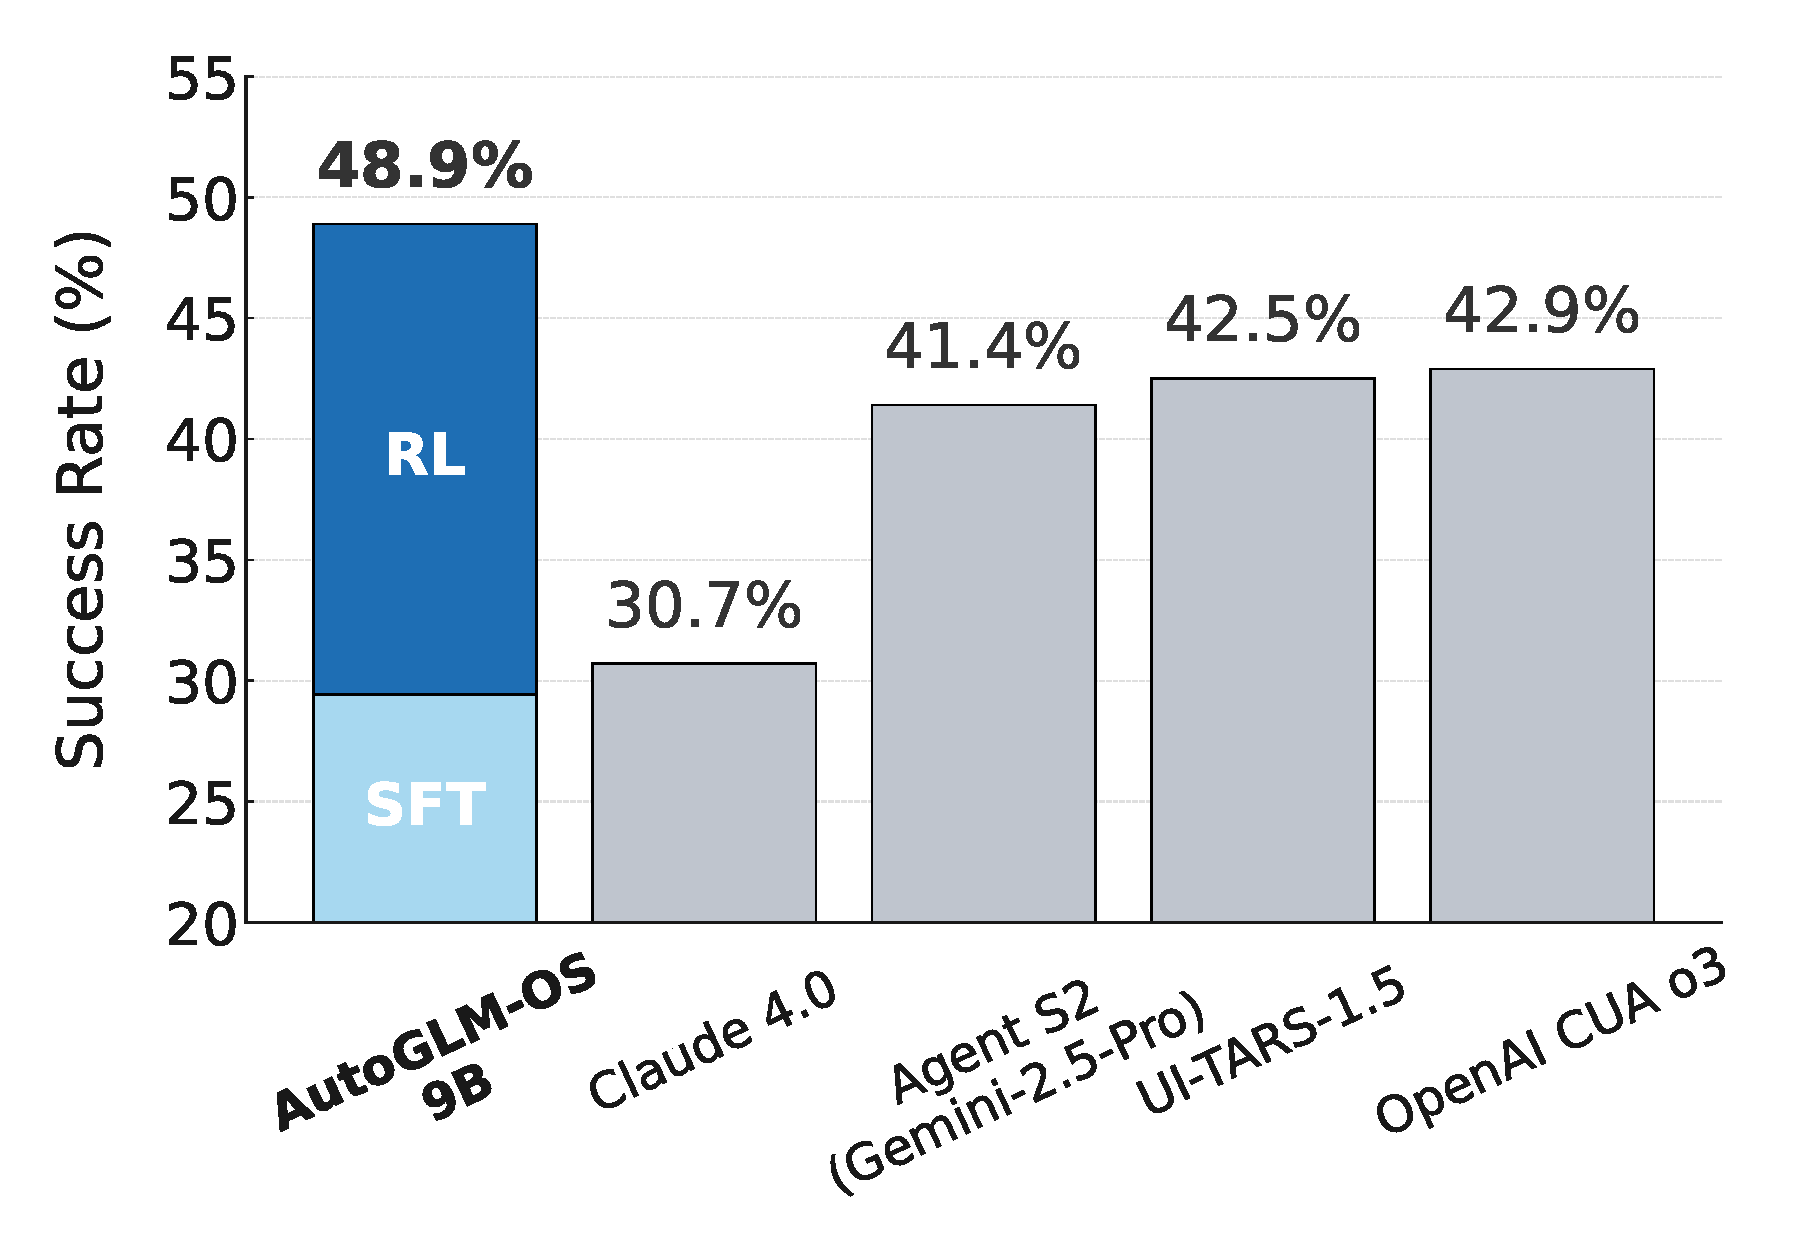
\includegraphics[width=\linewidth]{images/success_rates.pdf}
        \vspace{-7mm}
        \caption{The success rates of agents on OSWorld.}
        \label{figs:success_rate}
    \end{subfigure}
    \hfill
    \begin{subfigure}[t]{0.48\linewidth}
        \centering
        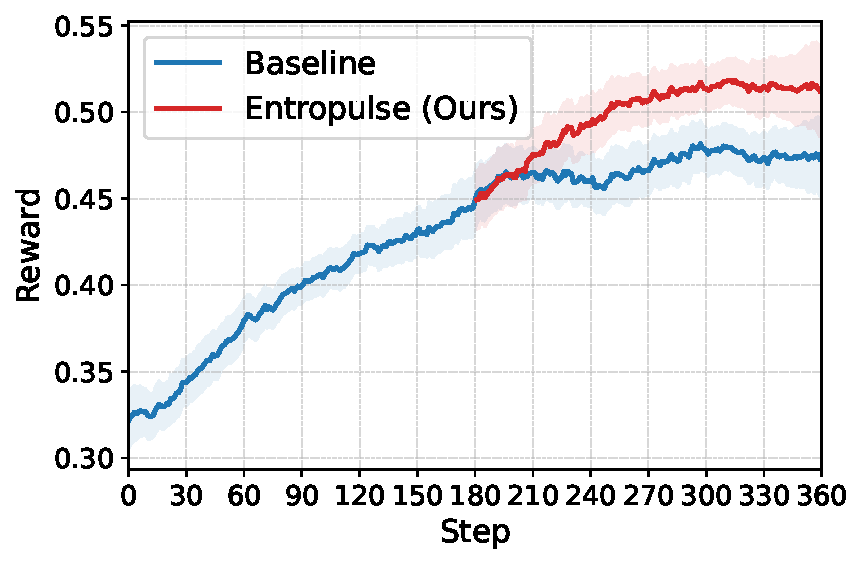
\includegraphics[width=\linewidth]{images/rl_curve_reward_intro.pdf}
        \vspace{-7mm}
        \caption{\computerrl training reward curves (95\% CIs).}
        \label{figs:trending-right}
    \end{subfigure}
    \vspace{-2mm}
    \caption{\computerrl enables efficient end-to-end online policy optimization for OS agents. (a) On OSWorld~\citep{xie2024osworld}, \model, trained with \computerrl, outperforms state-of-the-art agents. (b) Our \rlmethod approach yields higher average training rewards and improves both learning efficiency and final performance over conventional methods.}
    % \label{figs:trending}
\end{figure}

\begin{figure}[t!]
    \centering
    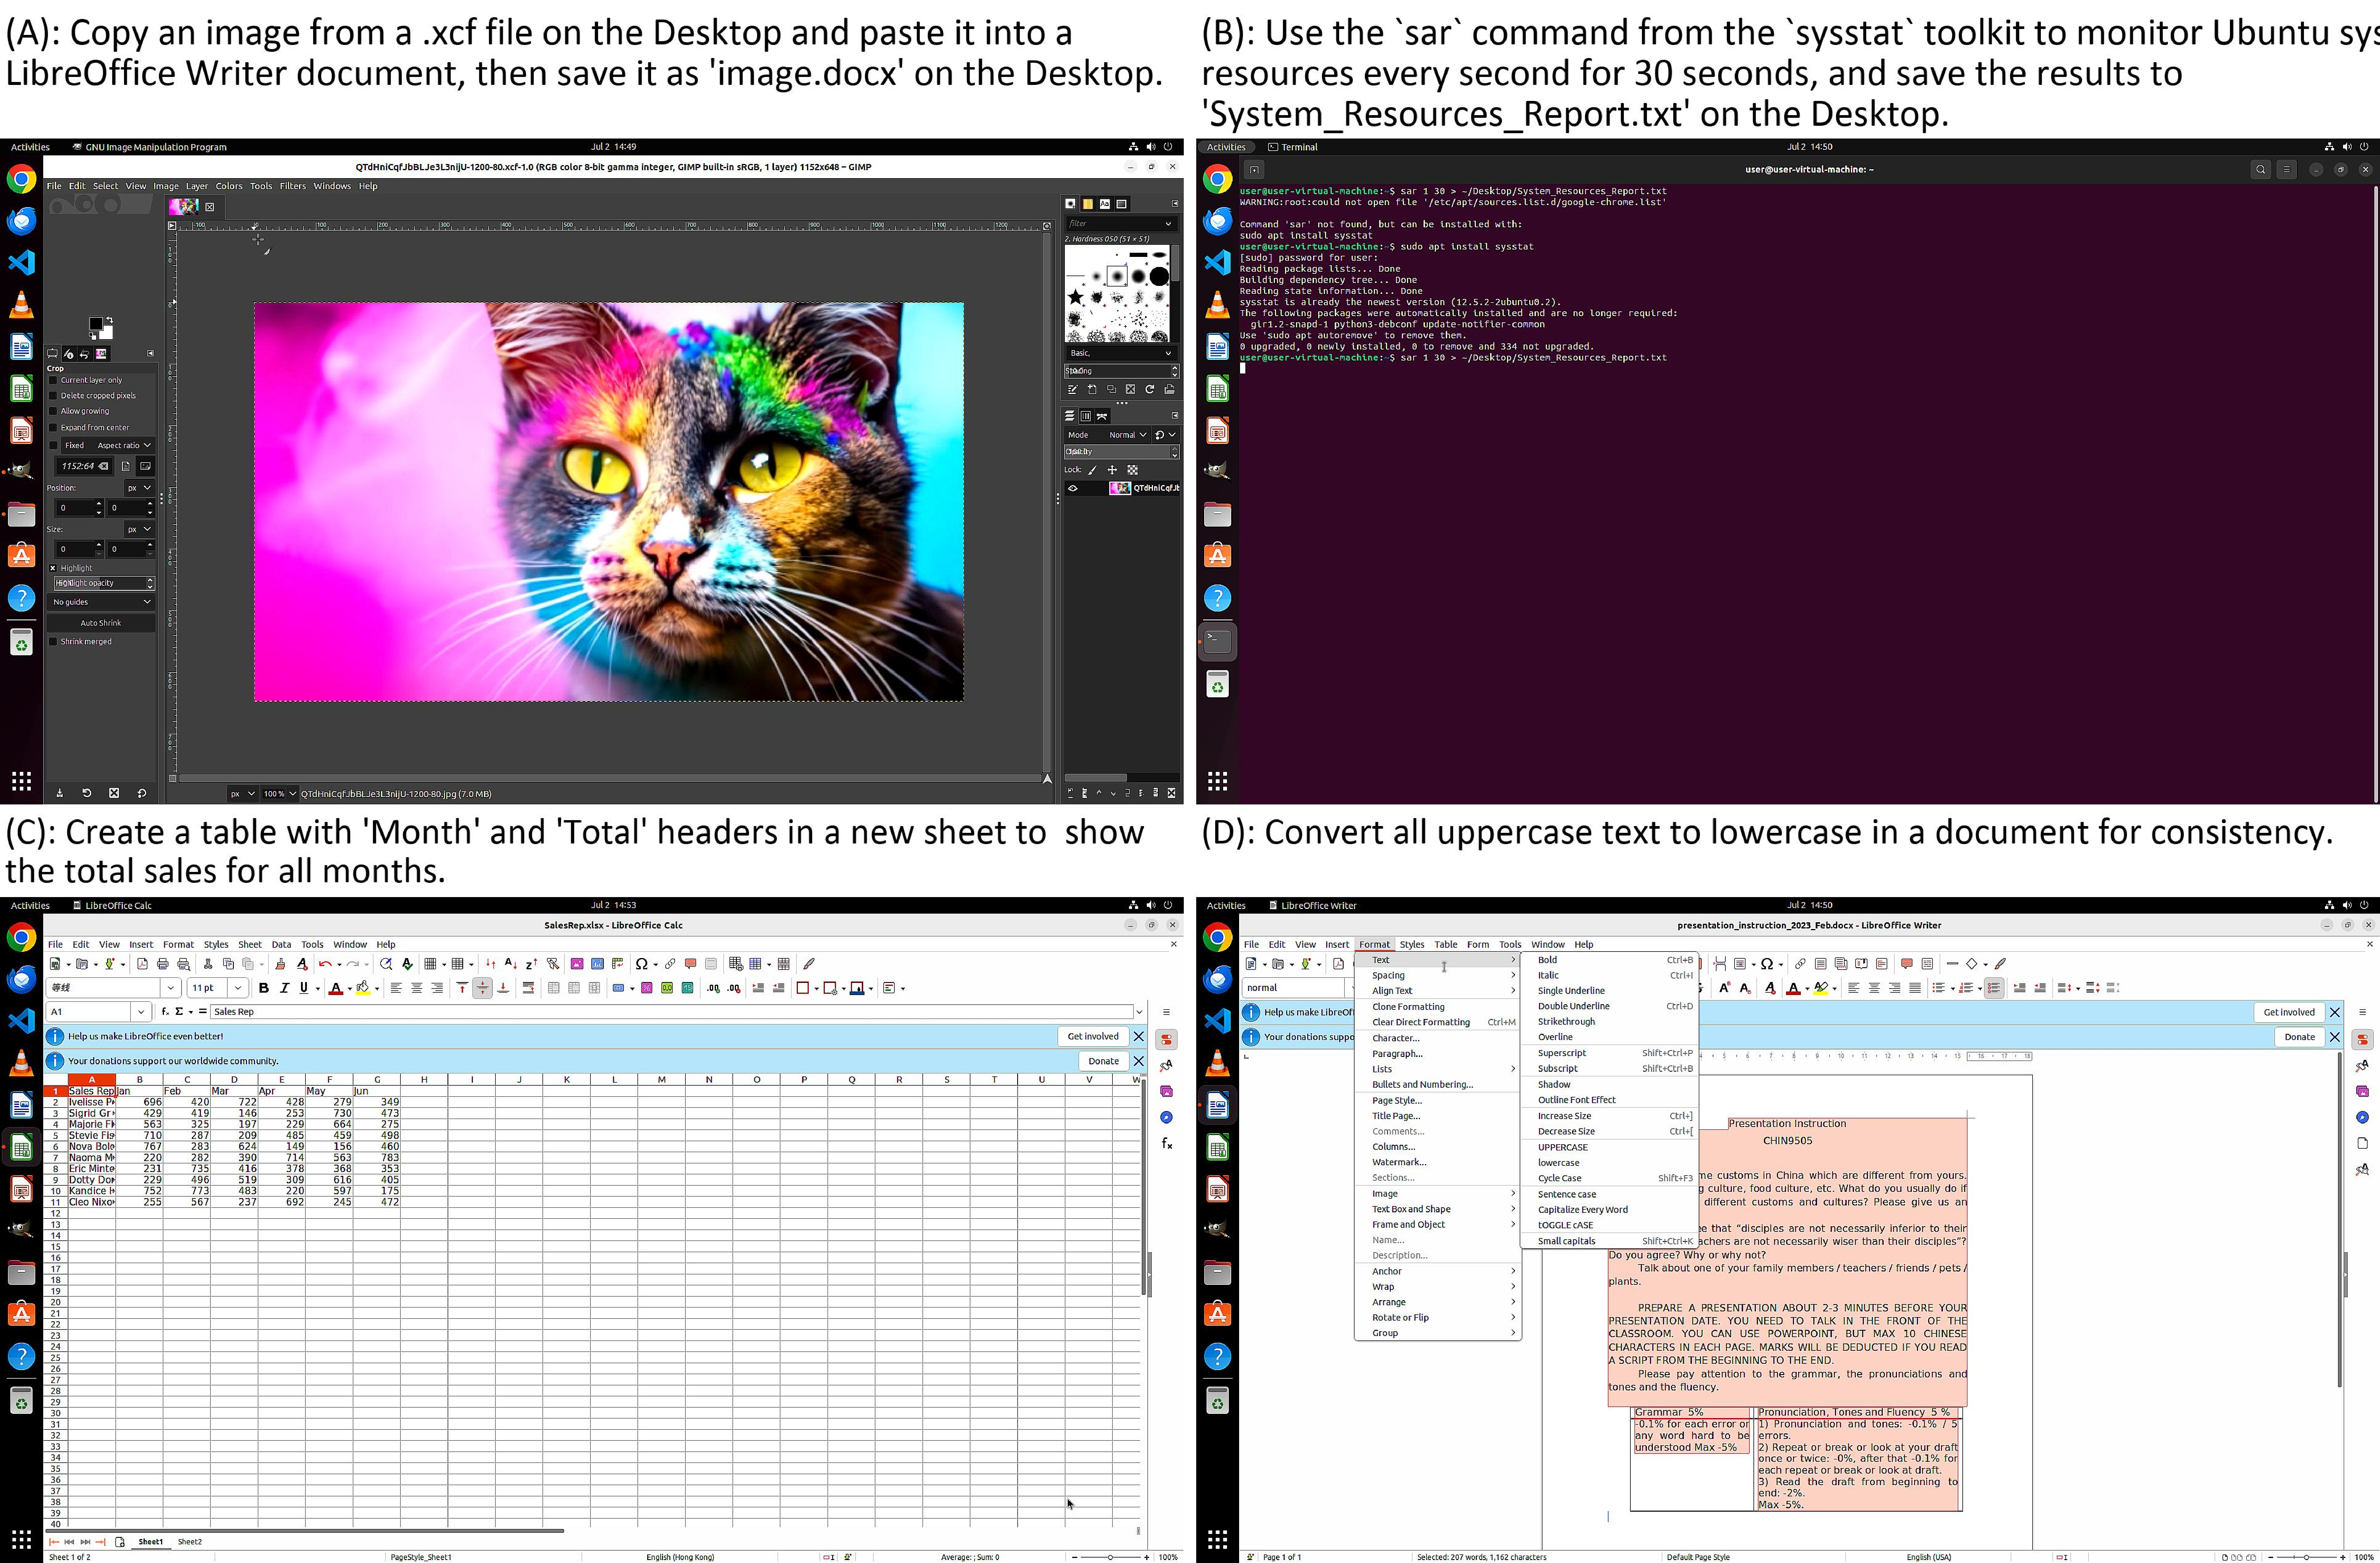
\includegraphics[width=1.0\linewidth]{images/shoutu.pdf}
    \vspace{-3mm}
    \caption{Examples of \model's execution on four user tasks, including image processing between GIMP and LibreOffice Writer, monitoring system resource usage in Terminal, table calculation in LibreOffice Calc, and document formatting in LibreOffice Writer.}
\end{figure}

\section{Introduction}
Large Language Models (LLMs)~\citep{achiam2023gpt, touvron2023llama2, zeng2022glm, glm2024chatglm, team2023gemini, guo2025deepseek, bai2023qwen, yang2025qwen3} have dramatically expanded the scope and depth of artificial intelligence capabilities, driving a profound re-examination of our understanding of machine intelligence.
Among all scenarios, the emergence of LLM-based GUI (graphical user interface) agents, capable of independently perceiving, reasoning, and executing complex tasks on user devices, has aroused particular interest from researchers~\citep{xi2023rise,wang2023survey,liu2023agentbench}. Given that desktops remain central to intelligence-intensive tasks, developing computer use agents is crucial for fundamentally transforming human-computer interactions and elevating AI capabilities~\citep{agashe2025agent, wu2024copilot}.

Despite previous attempts to develop computer use agents~\citep{agashe2025agent, lei2024infant, xie2025scaling}, enabling them to operate autonomously over extended periods in real-world scenarios remains a significant challenge. The first primary obstacle arises from the fact that GUIs are inherently designed for human interaction, making the simulation of human actions by GUI agents~\citep{liu2024autoglm,cua2025,qin2025ui} a non-trivial and cumbersome endeavor. 
Second, current mainstream approaches of behavior cloning (BC)~\citep{bain1995framework, bratko1995behavioural}, including manual annotation~\citep{he2025efficient} and model distillation~\citep{sun2024genesis,xu2024aguvis}, are limited in scalability and effectiveness. Manual annotation, while precise, is prohibitively labor-intensive for complex tasks. Model distillation, on the other hand, is constrained by the performance of the teacher models, limiting overall capability. Both methods typically exhibit poor generalization and limited error recovery abilities.
Finally, although reinforcement learning (RL) has shown potential for desktop automation tasks~\citep{lu2025arpo, feng2025group}, its practical application remains restricted due to computational complexity and methodological challenges. Complex environments, slow convergence, and known inefficiencies in RL training~\citep{xie2024osworld, bonatti2024windows, yu2025dapo, fu2025areal} severely limit its large-scale adoption in training computer use agents.

In this work, we propose \computerrl, an end-to-end algorithmic framework designed to advance desktop-level planning, reasoning, and device operation. This framework includes a new API-GUI interaction paradigm, a scalable RL training infrastructure for computer environments, and an RL algorithm for extended effective training.
First, we introduce \actionmethod, a large-scale, automatically constructed API ecosystem that enables the agent to transcend the inherent biases of human-oriented operational paradigms.
It instead leverages a more machine-oriented approach for device interaction, which combines API calls and GUI actions, thereby significantly enhancing both the versatility and overall performance of the agent.
Second, we develop a distributed training infrastructure utilizing virtual machine clusters based on Docker and gRPC protocols for scalability, which is fully compatible with AgentBench~\citep{liu2023agentbench}. This infrastructure supports \textbf{thousands of parallel environments}, ensuring high scalability and consistent interactions across all environments. Additionally, we integrate the training infrastructure with the AgentRL framework~\citep{zhang2025model} to facilitate efficient asynchronous training, thereby accelerating the training process.
Finally, to counteract stagnation and convergence issues in RL training—specifically, entropy collapse and rising KL divergence—we propose \rlmethod, which alternates between RL and SFT phases periodically. This approach maintains exploratory capacity and ensures continuous performance gains (Figure~\ref{figs:trending-right}). 

As a result, by harnessing end-to-end RL and optimization in the desktop environment, \computerrl has achieved remarkable improvement in understanding and operating GUIs. Evaluation on the OSWorld benchmark~\citep{xie2024osworld} shows \computerrl's significant improvements (see Figure~\ref{figs:success_rate}) in computer use challenges, achieving a success rate of \textbf{48.9\%} (with 66\% performance gain from RL), outperforming other state-of-the-art models including OpenAI CUA o3 (42.9\%), UI-TARS-1.5 (42.5\%), and Anthropic Claude Sonnet 4 (30.7\%).


In summary, our contributions are as follows:
\begin{itemize}[leftmargin=*,itemsep=0pt,parsep=0.2em,topsep=0.2em,partopsep=0.0em]
    \item We propose a new interaction paradigm, a shift from human-centric to machine-oriented interaction by introducing a large-scale, automatically constructed API ecosystem integrated with conventional GUI operations. This approach addresses the inherent mismatch between human-designed interfaces and artificial agent capabilities, while achieving superior operational efficiency and generalization performance on computer-based tasks.
    \item We establish a large-scale, distributed RL infrastructure for computer use agents by reconstructing virtual machine clusters, achieving unprecedented scalability with thousands of parallel environments and seamless AgentBench compatibility, thereby overcoming the critical bottleneck that has limited RL-based computer use agent training to scale experiments and enabling breakthrough results in large-scale agent training.
    \item We introduce \rlmethod, a novel training methodology that systematically addresses the challenges of entropy collapse and KL divergence accumulation in extended RL training through strategic alternation between RL and SFT phases, enabling sustained performance improvements and achieving state-of-the-art performance in computer automation.
\end{itemize}